%\section{Tools}
\subsection{Scala}
\label{sec:scala}
Scala is a programming language that combines the power of Object-oriented and functional programming. It was created by Martin Odersky in 2004 CITE. In his paper, An Overview of the Scala programming language, Odersky gives a good introduction to what Scala is 
\begin{quote}
	\textit{``Scala fuses object-oriented language and functional programming in a statically typed programming language. It is aimed at the construction of components of components and components system''}
	\begin{flushright}
		\cite{odersky2004overview}
	\end{flushright}		
\end{quote}

\subsubsection{Object-oriented}
Scala is object oriented because all values instantiated are objects and all operations performed are method calls. Scala does not have any primitive types, such as int, byte, boolean etc. In addition to all values being objects, all operators such as ``+, -, * , /'' etc. are function calls. Adding two numbers together $(x + y)$ can be written as ``x.+(y)''. Scala allows us to omit the dot notation and parentheses when the called function has exactly one input parameter. This is something that we will greatly benefit from when writing our DSL later in the project.
%http://www.scala-lang.org/old/sites/default/files/images/classhierarchy.img_assist_custom.png

\subsubsection{Functional}
Scala is a functional language because it supports the constructs needed for functional programming. Roughly described, functional programming implies that there are no variables or side-effects in a system. A function will always return the same result when it is called with the same input parameters. By using this definition we can call Java a functional language, it is however lacking certain core features. Namely treating functions as higher order functions. This implies that functions are values that can be  treated like any other value. They can be passed to functions, they can be the returned 
\\\\
The combination of these paradigms allows us to cherry pick the parts that we need for our solution and use the best of two worlds.
\\\\
Scala is run on the JVM and allows freely for the combination of both Scala and Java libraries. As a result of this Scala gains the benefits of having the mature Java ecosystem at its disposal. This is perhaps one of the reasons why Scala has seen a positive increase in its adoption rate. It enables the usage of the existing Java code without the need for re-implementing the entire system in Scala.

\subsubsection{Creating a DSL with Scala}
Scala however offers us the ability to write an embedded domain specific language. The main difference between a DSL and a embedded DSL is that the domain specific language is valid Scala code. This allows us to avoid the effort of needing to creating our own grammar and parser. 

Often when writing a DSL, we want to use a language that both feels and looks natural. Semi-colons, parenthesis and the dot-notation can make a language seem less natural. It also limits readability as it often does not provide any additional information. We find that ``a + b'' is much more readable than ``a.+(b)''. When creating our DSL we will therefor want to omit these characters when possible. It is however important to include parentheses when one wants to be explicit about precedence. ``a + b * c'' could be re-written as ``a + (b * c)'' to clearly show precedence.

A powerful feature of Scala the ``implicit'' construct. It allows us to implicitly pass values to functions. We can reduce redundancy and remove unneeded redundancy. When a function declares one of its input parameters as implicit, it will search the local scope for a value that has been declared with the keyword ``implicit''. During compilation of the system, the compiler will add the implicit values to the function call parameters.

\subsection{Case Classes}
Scala is capable of creating a ``plain-old-Java-object''(POJO) in just one line of code. It removes a lot of the boiler plate normally needed when creating a class. Methods such as constructors, getters/setters, toString etc. are created for us.

Case classes are meant to be used as data storing objects, a wrapper class. Unlike normal classes, a case class does not have any user-defined functions that can be added to it. It is mainly used for pattern matching operations.

\subsection{Akka} 
%REF: Need to cite more directly to akka.io or rewrite
Akka\footnote{akka.io}\cite{akka-documentation} is a toolkit designed specifically for implementing the Actor model. The Actor model approach to solving concurrency has been used by the Erlang language. Erlang has been used by the telecom industry to produce distributed and fault tolerant systems. 

\begin{figure}[h]
	\centering
	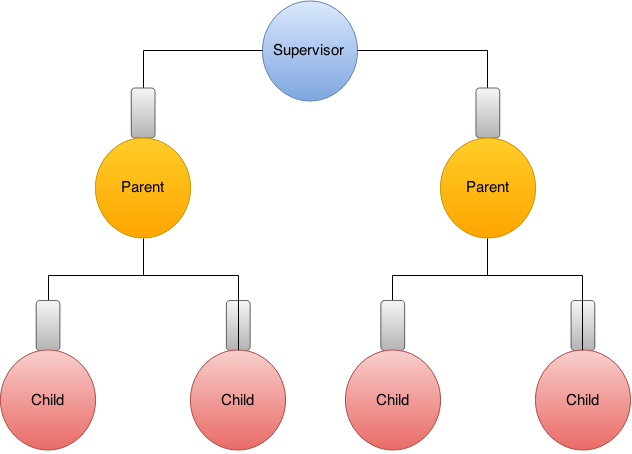
\includegraphics[scale=0.4]{images/tools/ActorModel.png} 
	\caption{Actor Model}
	\label{fig:ActorModel}
\end{figure}
\subsubsection{Actor Model}
The key points of the Actor model is building a hierarchy of  actors that receive messages in their mailbox. Figure \ref{fig:ActorModel} shows the general idea of the actors. The actors have a supervisor that will deliver tasks/messages to their inbox. The actors will then process the messages from their inbox and perform the appropriate task for each message. 
\subsubsection{Akka Actors}
The Actors in Akka are defined by Akka as lightweight, concurrent entities that use an event driven receive loop to process messages in its mailbox. An actors main functions can be boiled down to either receiving or sending messages. Akka's official documentation state that the size of a single actor is 300KB. With 1GB of heap memory, we can create approximately 2.5 million actors. 

These actors may share a thread or operate on different threads. We as developers do not need to worry about this as it is handled by the toolkit.
\\\\
The way the actors determine the appropriate response to a message is by using pattern matching. Pattern matching in short checks if the given message conforms to a certain pattern. This matching can be on the type of the message (int, string, boolean etc.) or on the actual value of the message (1, ``text'', true). By using this we can raise abstraction on how an actor will operate. Pattern matching greatly reduces the clutter that many ``if'' statements can create.
\\\\
Akke also has a feature that enables it to change its state, much like we would expect a protocol to do. It can changes its state to simulate the state of the protocol. This allows us to better understand how our actor will operate through its life cycle.
\begin{figure}[h]
	\centering
	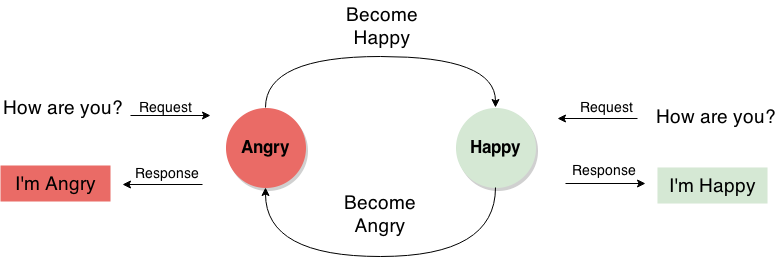
\includegraphics[scale=0.45]{images/tools/ActorState.png} 
	\caption{Actor State showing response to messages}
	\label{fig:ActorState}
\end{figure}
A simple state transition between ``Happy'' and ``Angry'' can be seen in figure \ref{fig:ActorState}. Depending on the state the actor is in, it will respond with a different message. In figure \ref{fig:ActorState} we can see that the response generated from a request is dependent on the state of the actor.

%REF:
%Scala Booker http://www.artima.com/pins1ed/a-scalable-language.html 
%Actor Model http://ieeexplore.ieee.org/xpls/abs_all.jsp?arnumber=886427&tag=1

